\subsection{Prologue}
When exposing \ce{Be+} and \ce{C+} in the ion trap to \ce{H2O} vapor introduced from the leak valve, we found that the reaction \ce{Be+ +H2O -> BeOH+ + H} occurs. Interestingly, it occurred at a slower rate than that of \ce{C+ + H2O}, where by ADO, the rates should be nearly indistinguishable. Towards our goal of understanding \ce{C+ + H2O}, we needed to understand the role that \ce{Be+} may have, as all of the charged reaction products will stay in the trap. Along the way, we gained a fuller understanding of the \ce{Be+ + H2O} reaction, which proved to be an invaluable tool for subsequent studies. The rate constant was both experimentally and theoretically found to be excited state dependent, despite the fact that both reaction pathways are exothermic. Knowing this rate constant to a high degree of confidence allowed us to characterize the water density at the ion trap from the CBGB, which neither our RGA nor ion gauge could detect.

\subsection{Introduction}
Low-temperature reactions of simple ions with small molecules play a central role in astrochemical environments from interstellar clouds to cometary comae to planetary atmospheres, including that of Earth\cite{Agundez2013,Krasnopolsky2014}. The chemical evolution of interstellar molecular clouds ultimately yields the seedbed from which new stars and planets are born and the raw materials from which life likely developed. A firm understanding of the reaction rates for a host of elementary ion-molecule reactions is essential to accurately model these environments these environments. Techniques such as selected ion flow tubes (SIFTs)\cite{Adams1976}, guided ion beams\cite{Armentrout2002}, and supersonic flows (CRESU)\cite{Sims2002} have improved our empirical understanding of these processes; however, each has its own limitations.\cite{Smith2000,Snow2008} Theoretically, it has long been recognized that these ion-molecule reactions are often barrierless, and their rates are frequently described by capture models.\cite{Gioumousis1958a} However, recent studies have revealed that dynamical features can sometimes prevail,\cite{Lourderaj2008,Li2014,Carrascosa2017} in which case statistical treatments may not be accurate.\cite{Hase2014,Clary1990} Therefore, new experimental and theoretical efforts are needed to accurately address ion-molecule chemistry. Furthermore, there have been very few experimental studies of gas-phase reactions between metal ions and water, especially at low temperature, despite their importance for metal ion chemistry in a range of environments.\cite{Highberger2001,Oppenheimer2002,VanDishoeck2013a}

Singly ionized beryllium is a particularly attractive metallic reactant to use for such studies because it is both theoretically tractable and experimentally highly controllable. The relatively simple electronic structure of this three-electron ion allows both highly accurate characterization of its electronic structure and laser cooling,\cite{Bollinger1985} and the low mass of \ce{Be+} lends itself to high motional frequencies as well as efficient sympathetic cooling of other chemically interesting atomic ions when employed in ion traps.\cite{Chen2014a,Roth2006,Larson1986,Schowalter2016} For the molecular reaction partner, \ce{H2O} is arguably the most important molecule in chemistry, and theoretical studies of its reactions with a single atom have been reported on full-dimensional potential energy surfaces (PESs).\cite{Li2013,Song2015,Ray2017,Li2015,Xiao2011} Thus this system of reagents provides an opportunity to perform a high-resolution comparison between experiments and theory for a molecule-ion system.

\subsection{Experimental}

To study the \ce{Be+ + H2O} reaction, \ce{Be+} was loaded into the trap and cooled with the 313 nm laser, then exposed to \ce{H2O} vapor introduced from the leak valve.

To minimize experimental errors, a combination of fluorescence detection and TOF measurements were used in tandem. Using both methods together, compared to only using the TOF, allows us to cut down the data collection time, which greatly reduces the effects of drifts in laser power and locking. The initial fluorescence signal determines the reaction time zero as well as normalize the initial ion number for the TOF traces. TOF traces are taken at various reaction times to determine the relative reaction product signals via shared fitting of solved differential equations including all possible reaction pathways shown in Figure \ref{fig: Be+H2O shared fit}. In total, we consider the following 8 reaction pathways, all of which are thermochemically allowed.

\begin{align}
	\ce{Be+(^2S1/2) + H2O & -> BeOH+ + H} \label{r: Be(S)+H2O->BeOH} \\
	\ce{Be+(^2P3/2) + H2O & -> BeOH+ + H} \label{r: Be(P)+H2O->BeOH} \\
	\ce{Be+(^2P3/2) + H2O & -> H2O+ + Be} \label{r: Be(P)+H2O->H2O} \\
	\ce{H2O + H2O+ & -> H3O+ + OH} \label{r: H2O+H2O->H3O} \\
	\ce{Be+(^2P3/2) + H2O & -> BeH+ + O2} \label{r: Be(P)+H2O->BeH} \\
	\ce{BeH+ + H2O & -> BeOH+ + H2} \label{r: BeH+H2O->BeOH} \\
	\ce{Be+(^2P3/2) + H2O & -> BeO+ + H2} \label{r: Be(P)+H2O->BeO} \\
	\ce{BeO+ + H2O & -> BeOH+ + OH} \label{r: BeO+H2O->BeOH}
\end{align}

Typical TOF traces (10 sample average) at reaction times $t=0$ and 70 s with 7 and 26\% relative \ce{Be+(^2P3/2)} state excitation are shown in Figure 1A,B, respectively. At $t=0$ s, a large peak of $m/z=9$(\ce{Be+}) and a smaller one of $m/z=9$(\ce{BeOH+}) are evidenced in the TOF trace (blue line), which indicates that \ce{Be+} ions are the main species in the trap at $t=0$. The finite amount of \ce{BeOH+} at $t=0$ reflects the fact that reactions \ref{r: Be(S)+H2O->BeOH}-\ref{r: BeO+H2O->BeOH} happen even during the loading process and that the A-ramp mass filtering procedure is imperfect. At $t=70$ s, a $m/z=19$ peak emerges when more \ce{Be+} ions are excited to \ce{^2P3/2} state (figure \ref{fig: Be+H2O TOF}), which we identify as \ce{H3O+} resulting from reactions \ref{r: Be(P)+H2O->H2O}and \ref{r: H2O+H2O->H3O}. The \ce{BeOH+ / H3O+} ratio, $\eta(P_\text{P})$, is measured by integrating both peaks for the experimentally controlled excited-state population $P_\text{P}$. The \ce{BeOH+} signal includes the amount unfiltered during loading, products from both reactions \ref{r: Be(S)+H2O->BeOH} and \ref{r: Be(P)+H2O->BeOH}, as well as, in principle, the two-step reactions \ref{r: Be(P)+H2O->BeH},\ref{r: BeH+H2O->BeOH}\ref{r: Be(P)+H2O->BeO}, and \ref{r: BeO+H2O->BeOH}. The \ce{H3O+} signal is produced via the two-step reactions \ref{r: Be(P)+H2O->H2O}\ref{r: H2O+H2O->H3O}. Whereas we do not observe products from reactions \ref{r: Be(P)+H2O->BeH}, \ref{r: BeH+H2O->BeOH}, \ref{r: Be(P)+H2O->BeO}, or \ref{r: BeO+H2O->BeOH} (see Figure \ref{fig: Be+H2O shared fit}). They are thermochemically allowed and therefore included in our analysis, which sets upper limits on their reaction rate coefficients.

\begin{figure}
	\centering
	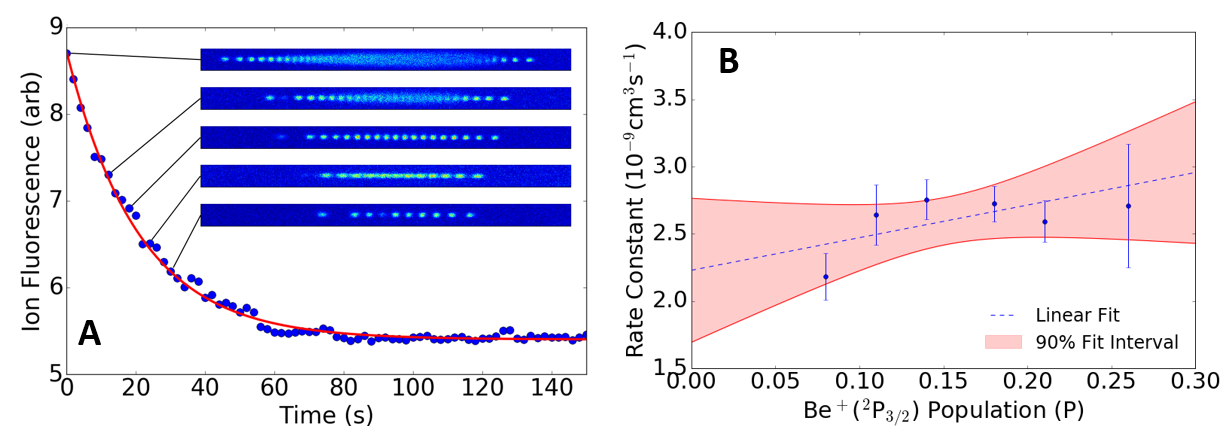
\includegraphics[width=\textwidth]{images/Be_H2O_fit.png}
	\caption{(A) Typical fluorescence decay measurement. The inset images are a subset of the original ion fluorescence images recorded by the camera. The red curve is an exponential fit (with a free offset) to the data, which gives the total reaction rate. (B) Total reaction rate coefficient as a function of \ce{Be+ (^2P3/2)} state population can be used to separate the contributions from the ground and excited states of \ce{Be+.}}
	\label{fig: Be+H2O fit}
\end{figure}

\subsection{Results and Discussion}

The total reaction rate is given by $\Gamma_t = \rho_{\ce{H2O}} k_t$, where $\rho_{\ce{H2O}}$ is the \ce{H2O} density measured the RGA calibrated to the ion gauge (section \ref{sec: calibration}) and $k_t$ is approximated as $k_t = P_\text{S} k_1 + P_\text{P} k_2 + P_\text{P} k_3$, where $P_\text{S}$ and $P_\text{P}$ are the \ce{Be+} population in the \ce{^2S1/2} and \ce{^2P3/2} states, respectively, and $k_i$ is the reaction rate coefficient of reaction $i$. Reaction \cref{r: H2O+H2O->H3O} has been studied by other groups, reporting a rate coefficient of $(2.05 \pm 0.010) \times 10^{-9}$ cm$^3$/s.\cite{Huntress2004} The measured \ce{H3O+ / BeOH+} ratio is given from the reaction rates by:

\begin{equation}
	\eta(P_\text{P}) = \frac{P_\text{P} k_3}{P_\text{S} k_1 + P_\text{P} k_2}
	\label{eq: eta=H3O/BeOH}
\end{equation}

To use equation \ref{eq: eta=H3O/BeOH} to extract the individual rate coefficients $(k_i)$, the total reaction rate $\Gamma_t$ is first measured by monitoring the \ce{Be+} fluorescence decay with a camera, as shown in Figure \ref{fig: Be+H2O fit}A. Fluorescence decay is monitored directly after a DC voltage applied to trap electrodes is used to filter out the heavier products from the trap to allow better crystallization of the \ce{Be+} ions by reducing ion-ion heating.\cite{Chen2013} The inset of Figure \ref{fig: Be+H2O fit}A shows typical fluorescence images of the \ce{Be+} coulomb crystal at various times. Fluorescence is used to measure the total reaction rate because the total measurement time is ~30 times shorter than using the TOFMS (Figure \ref{fig: Be+H2O shared fit}). To determine the separate rate coefficients for the \ce{Be+} ground and excited states, we measure the total reaction rate coefficients for different excited-state fractions, shown in Figure \ref{fig: Be+H2O TOF}. A linear fit (blue line) is found using the least-squares method. The vertical intercept of this fit gives the \ce{Be+} ground-state reaction rate coefficient $k_{\ref{r: Be(S)+H2O->BeOH}}=(2.2 \pm 0.3_{stat}) \times 10^{-9}$ cm$^3/$s, whereas the sum of the slope and intercept gives the total excited-state \ce{Be+} reaction rate coefficients $k_{\ref{r: Be(P)+H2O->BeOH}} + k_{\ref{r: Be(P)+H2O->H2O}} = (4.7 \pm 1.7_{stat}) \times 10^{-9}$ cm$^{-3}$/s. Using equation \ref{eq: eta=H3O/BeOH}, the reaction rate coefficients of reactions \ref{r: Be(P)+H2O->BeOH} and \ref{r: Be(P)+H2O->H2O} are then calculated to be $k_{\ref{r: Be(P)+H2O->BeOH}} = (4.2 \pm 1.6_{stat}) \times 10^{-9}$ cm$^{-3}$/s and $k_{\ref{r: Be(P)+H2O->H2O}} = (0.47 \pm 0.11_{stat}) \times 10^{-9}$ cm$^{-3}$/s, respectively. The ratio of reaction rate coefficients for reactions \ref{r: Be(P)+H2O->H2O} to \ref{r: Be(P)+H2O->BeOH} is therefore $k_{\ref{r: Be(P)+H2O->H2O}}/k_{\ref{r: Be(P)+H2O->BeOH}} = 0.11 \pm 0.03$ independent of systematic errors in the density measurement. Charged products from reactions \ref{r: Be(P)+H2O->BeH} and \ref{r: Be(P)+H2O->BeO} are not directly observed and an upper bound is found to be $<5\times10^{-10}$ cm$^3$/s, set by the integrated signal threshold. Reactions at these upper bounds for the rate coefficients do not significantly change the analysis above, justifying their exclusion from $k_i$.

It is instructive to compare these measured rate coefficients to those predicted by capture theory. Since the translational energy of the laser-cooled \ce{Be+} ions is $<0.5$ K, the energy of the room-temperature water sets the reaction kinetic energy of \ce{Be+ + H2O} in the center of mass frame of $~100$K. The internal state distribution of the \ce{H2O} is assumed to be given by the 300 K. The internal state distribution of the \ce{H2O} is assumed to be given by the 300 K. Because \ce{H2O} has a dipole, we use the ADO theory (equation \ref{eq: k ADO}) to estimate the rate constant. The ADO model predicts that both the ground and excited Be+ states react with a rate coefficient $k_{\text{ADO}} = 4.1 \times 10^{-9}$ cm$^3$/s at 100 K reaction temperature, roughly two times larger than measured for the ground state, but in agreement with the measured reaction rate of the excited state. Since the experimental rate constant agrees well with the theoretical rate, we may generalize \ref{r: Be(S)+H2O->BeOH} and \ref{r: Be(P)+H2O->BeOH} to:

\begin{equation}
	k_{\ref{r: Be(P)+H2O->BeOH}+\ref{r: Be(S)+H2O->BeOH}}(T) \approx ((0.54)k_{ADO}(P) + (0.49)k_{ADO}) \times 10^{-9}\text{ cm}^3/s
	\label{eq: k Be+H2O(T)}
\end{equation}

However, because it is long-range, the ADO model cannot provide the branching ratio and state-dependent information and is therefore insufficient for describing the observed reactions. Hua Guo at UNM helped us in making theoretical calculations on the reaction dynamics by method of Quasi-Classical Trajectory Calculations (QCT-Calculations) on a full-dimensional potential energy surface (PES).\cite{Yang2018} They calculate that the intermediate state (IM1) in Figure \ref{fig: Be+H2O PES} on the ground state reaction pathway causes about 46\% of the incoming trajectories to reflect back to the entrance channel yielding a rate constant $k_{\ref{r: Be(S)+H2O->BeOH} th} = (2.02 \pm 0.04) \times 10^{-9}$ cm$^3$/s. The excited state pathway does not have a submerged barrier of this level, but does have a nonadiabatic transition bringing it down to the ground state product channel.

\subsection{Conclusion}

In short, chemical reactions of laser-cooled \ce{Be+} ions with room-temperature water vapor have been studied experimentally and theoretically for the first time. Ground-state \ce{Be+} ions produce only \ce{BeOH+ + H} with a reaction rate coefficient of $k_{\ref{r: Be(S)+H2O->BeOH}} = (2.2 \pm 0.3_{\text{stat}}) \times 10^{−9}$ cm$^2$/s, whereas the excited-state \ce{Be+} not only creates \ce{BeOH+ + H} with a reaction rate coefficient of $k_{\ref{r: Be(P)+H2O->BeOH}} = (4.2 \pm 1.6_{\text{stat}}) \times 10^{−9}$ cm$^3$/s but also gives \ce{H2O+ + Be} with a reaction rate of $k_{\ref{r: Be(P)+H2O->H2O}} = (0.47 \pm 0.11_{\text{stat}}) \times 10^{-9}$ cm$^3$/s. Electronic structure calculations indicate that these two products are both produced via nonadiabatic pathways. The ground-state reaction rate is roughly half of that predicted by typically employed capture models but in good agreement with zero-point-corrected QCT calculations on an accurate full-dimensional global PES based on high-level ab initio calculations. These calculations reveal that the lower reaction rate is a consequence of chemical dynamics due to a submerged barrier in the product channel.

\begin{figure}
	\centering
	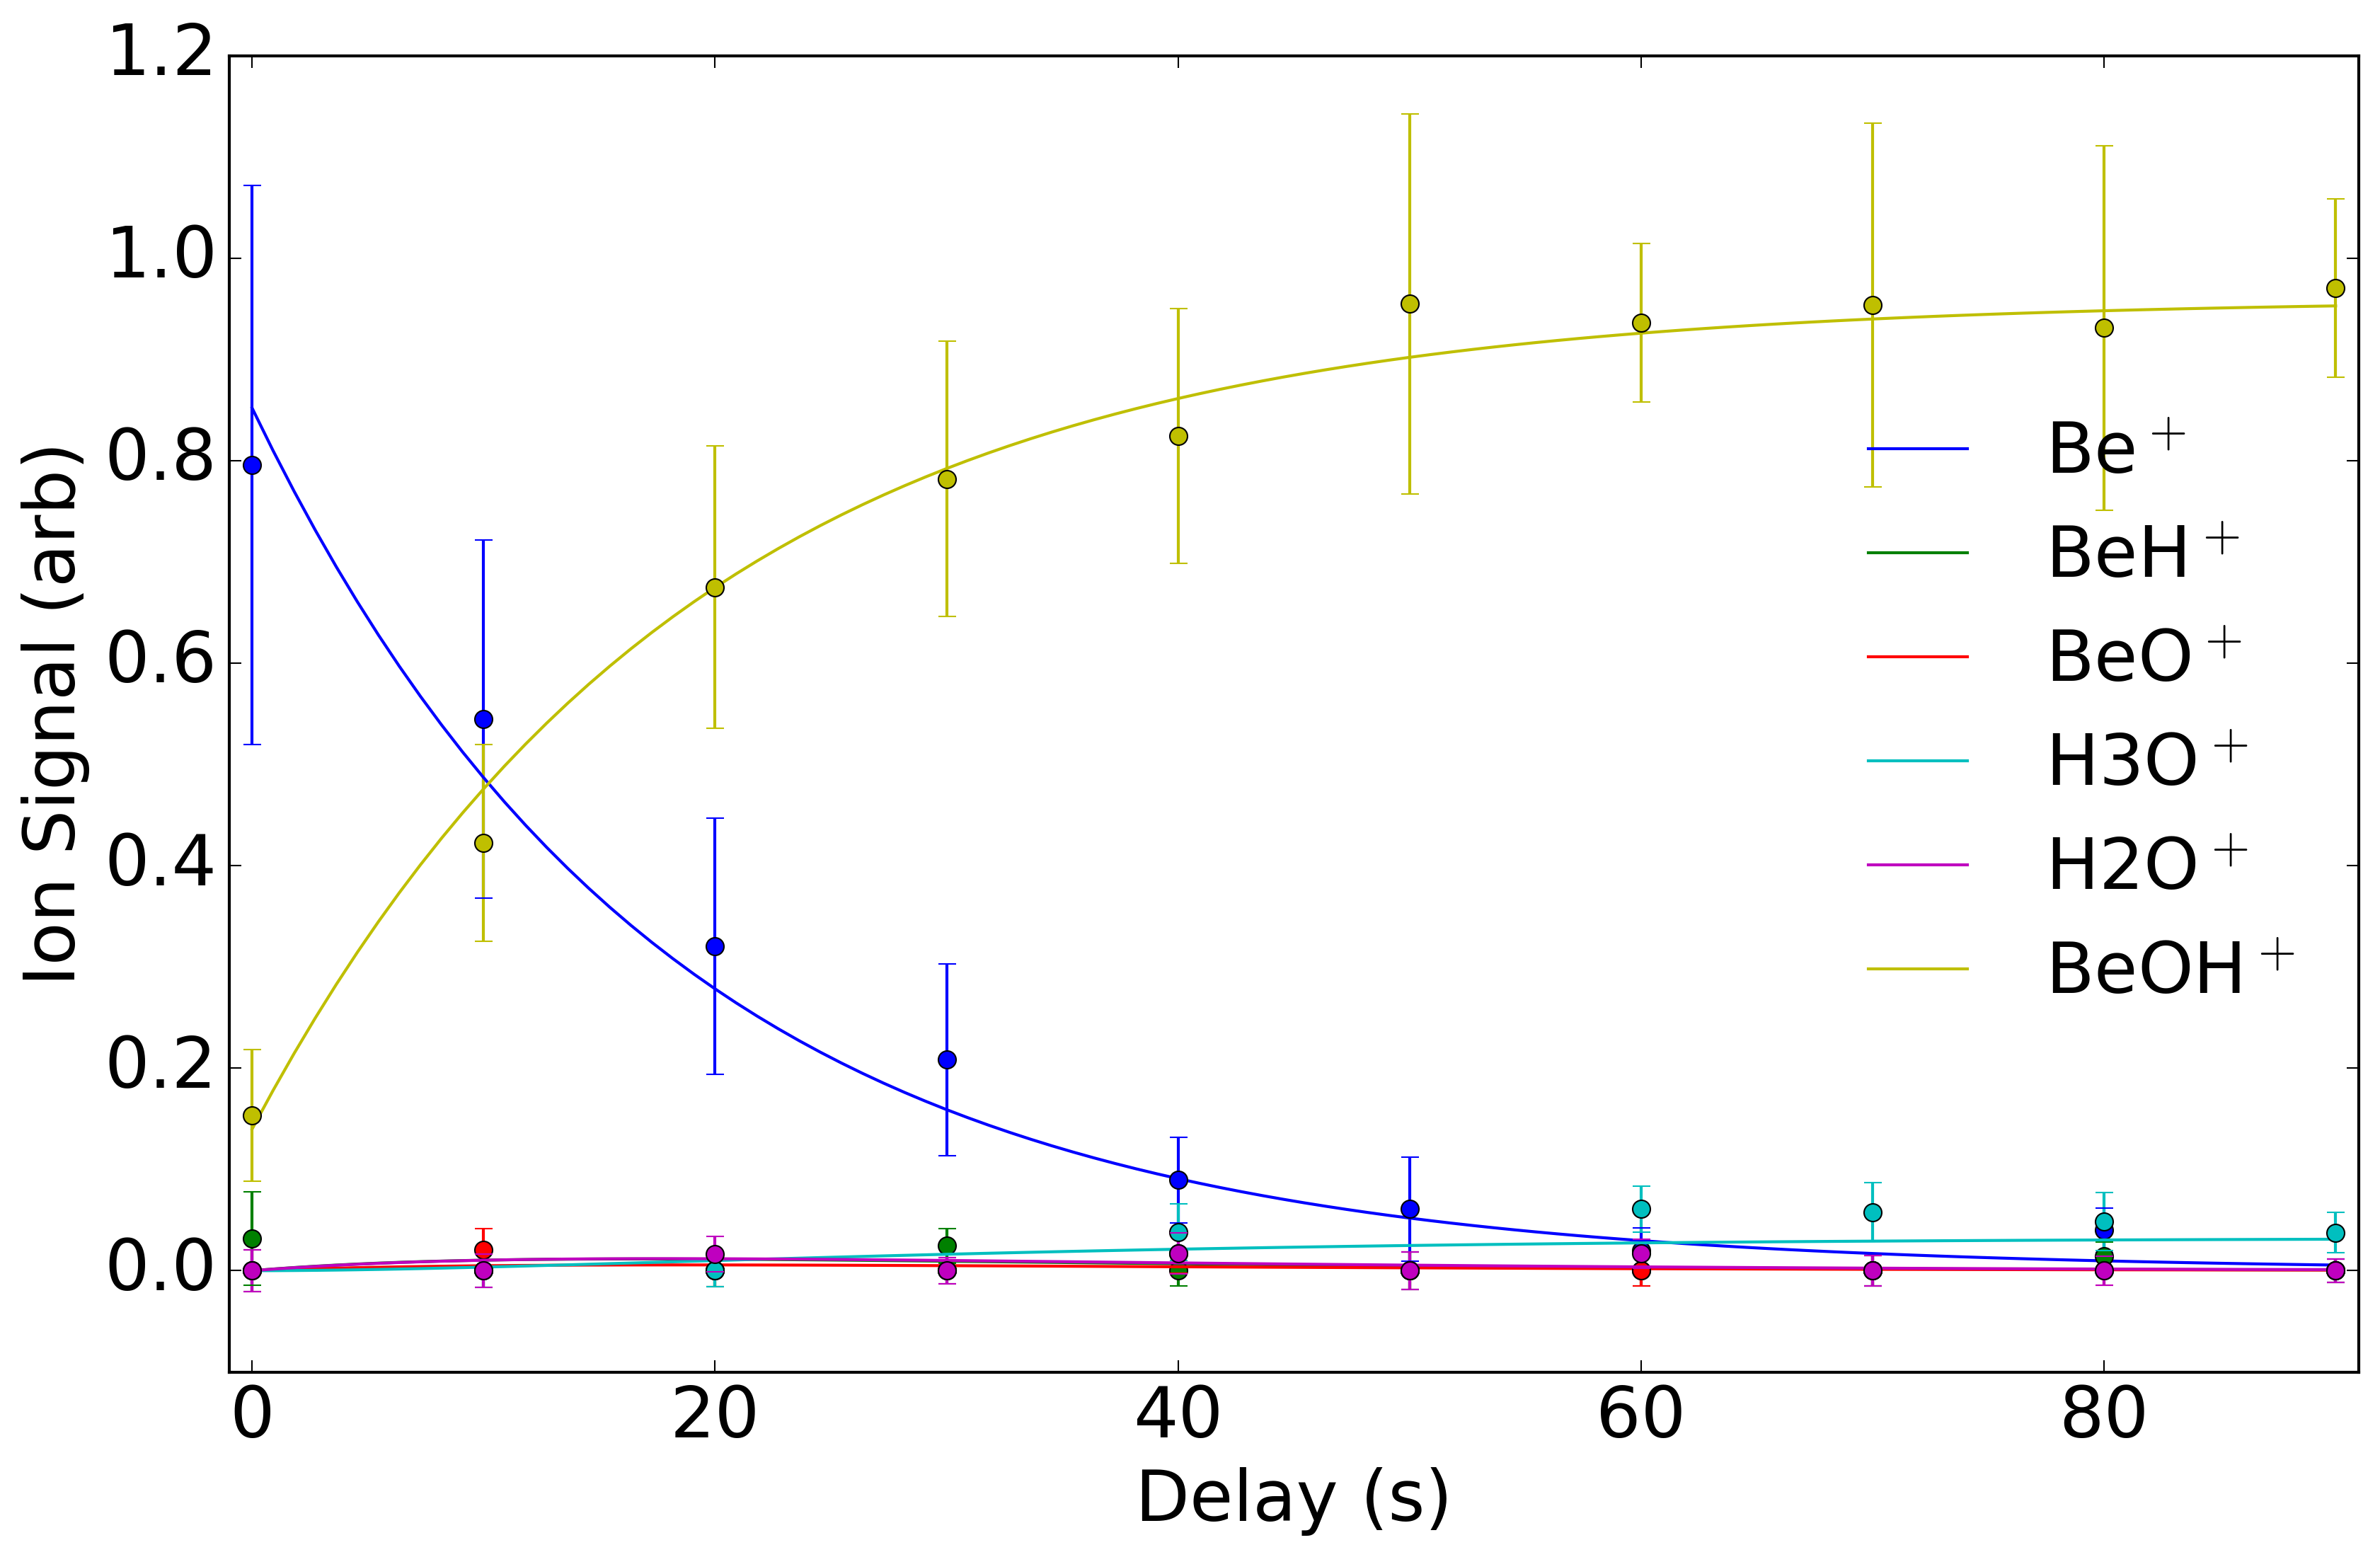
\includegraphics[width=0.8\textwidth]{images/Be_H2O_sf.png}
	\caption{The temporal evolution of \ce{Be+}	in the trap as a function of reaction time as well as the solutions of differential equations fitted to the kinetics data with $P_{\text{P}}$ = 26\%.}
	\label{fig: Be+H2O shared fit}
\end{figure}

\begin{figure}
	\centering
	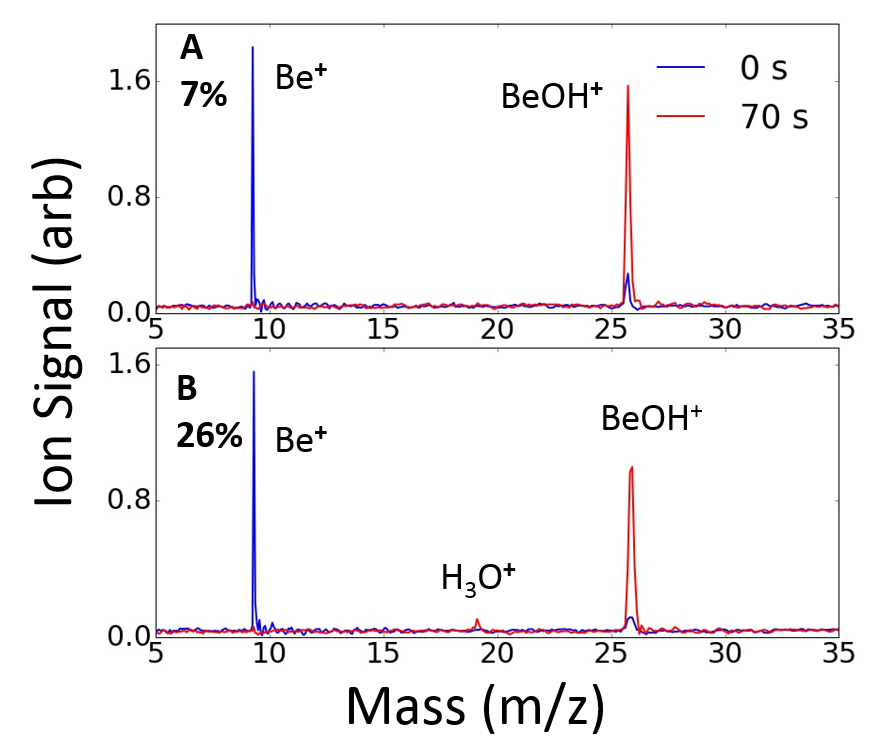
\includegraphics[width=0.8\textwidth]{images/Be_H2O_TOF.png}
	\caption{TOF signal (averaged over 10 trials) at reaction time $t = 0$ and 70 s with (A) $P_{\text{P}}$ = 7\% (A) and (B) $P_{\text{P}}$ = 26\%. A clear $m/z = 19$ peak emerges when more \ce{Be+} ions are excited to \ce{^2P3/2} state. The \ce{BeOH+ / H3O+} ratio for this case ($P_{\text{P}}$ = 26\%) is measured to be $\eta(0.26) = 0.039 \pm 0.006$ by integrating both peaks in B when $t = 70$ s.}
	\label{fig: Be+H2O TOF}
\end{figure}

\begin{figure}
	\centering
	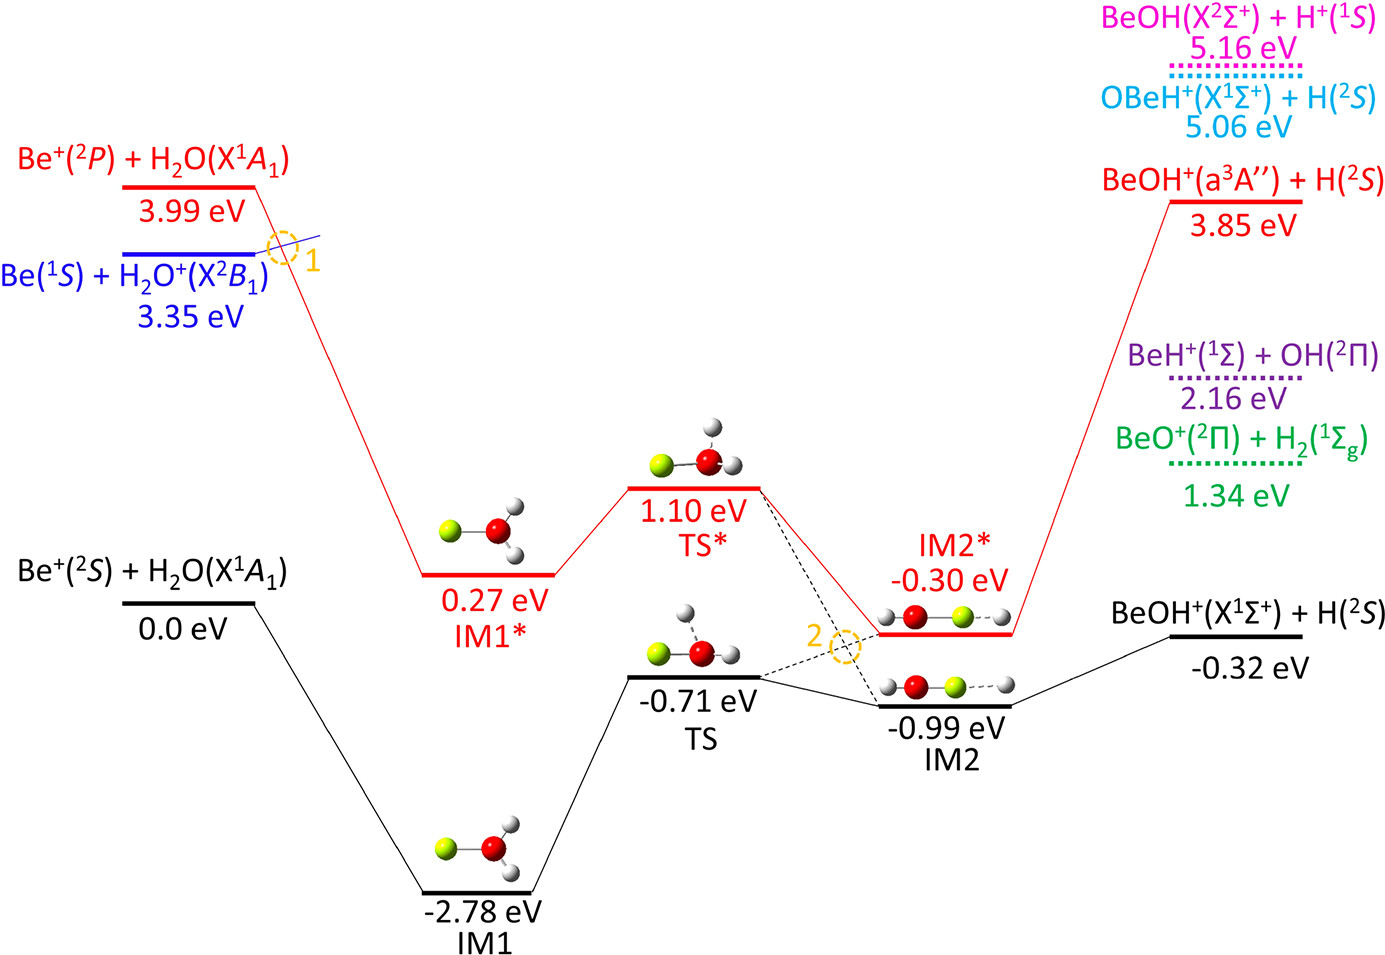
\includegraphics[width=0.8\textwidth]{images/Be_H2O_PES.jpeg}
	\caption{Energetics of both the ground- and excited-state reaction pathways for the \ce{Be+ + H2O} reaction. Whereas reaction \ref{r: Be(S)+H2O->BeOH} proceeds on a single adiabatic PES, the reactions involving excited \ce{Be+} depend on nonadiabatic transitions between different PESs (yellow circles). The submerged well on the ground-state reaction pathway prevents 46\% of the trajectories to reflect back to the entrance channel. (Taken from \cite{Yang2018})}
	\label{fig: Be+H2O PES}
\end{figure}

